\documentclass[12pt]{book}
\usepackage[utf8]{inputenc}
\usepackage{graphicx}
\usepackage{amsmath}
\usepackage{amssymb}

\title{Peculiaridades del Tono del Violín}
\author{Frederick Castle, M. D.}
\date{1906}

\begin{document}

\maketitle
\begin{center}
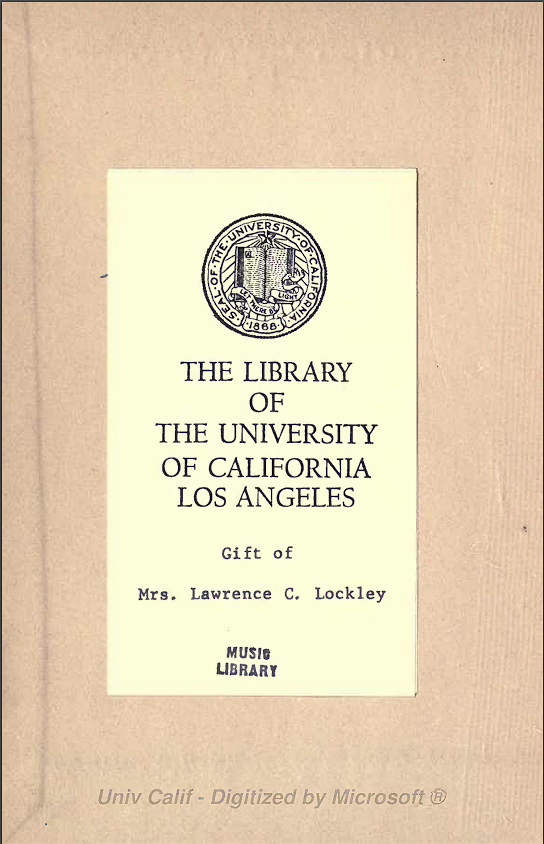
\includegraphics[width=1\textwidth]{./img/portada.png} % Reemplaza "imagen.jpg" con el nombre del archivo de la imagen
\end{center}
\begin{center}
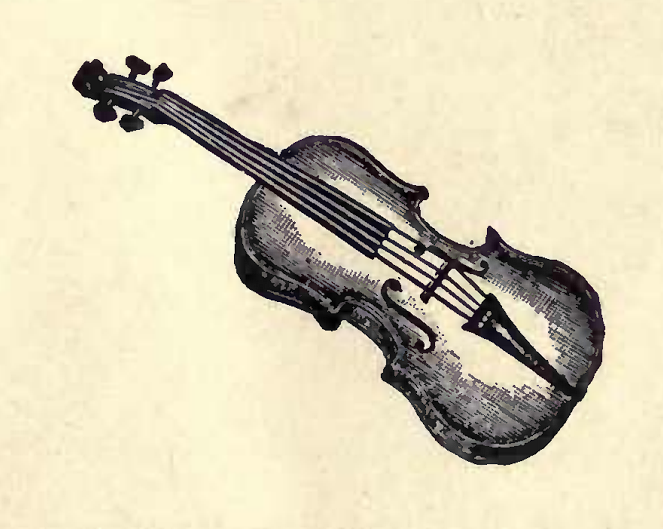
\includegraphics[width=0.5\textwidth]{./img/violin.png} % Reemplaza "imagen.jpg" con el nombre del archivo de la imagen
\end{center}

\begin{center}
\textbf{LOWELL, INDIANA.\\
Alfred Ha Miller}

\textbf{Copyright 1906,\\
Por Frederick Castle, M. D.\\
H. H. RAGON \& SON, Impresores,\\
Lowell, Indiana.\\
1906.}
\end{center}

\begin{center}
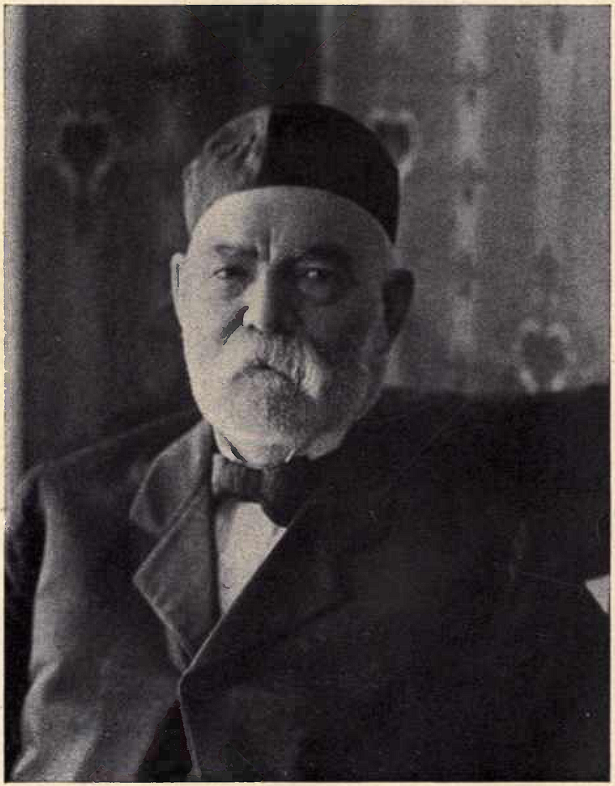
\includegraphics[width=1\textwidth]{./img/foto.png} % Reemplaza "imagen2.jpg" con el nombre del archivo de la imagen
\end{center}

\chapter*{Agradecimientos}

Es gratificante reconocer al Mayor Gilbert Thompson, Washington, D. C., y al Sr. Frank Spalding, Director del Municipio de Griffth, Indiana, como personas que brindaron una valiosa ayuda para hacer que este libro sea presentable.

\begin{flushright}
\textbf{FREDERICK CASTLE}
\end{flushright}

\chapter*{Explicación del Gráfico}

Debido a que diferentes muestras de madera para la tabla armónica deben recibir un tratamiento distinto en cuanto a graduación, no se dan valores para los espesores; pero en lugar de cifras, se emplea sombreado como medio para indicar valores cuantitativos relativos. El único experimento anotado en el texto, y que tiene en cuenta la uniformidad máxima del poder tonal, operó para aumentar las notas altísimas en un grado más marcado que los tonos de menor altura. Debido a que el poder en los tonos altísimos es deseable y difícil de asegurar, por lo tanto, se registra este método de graduación, con la esperanza de que futuros estudiantes del violín continúen experimentando con el acortamiento de la longitud de la actividad de la tabla armónica para aumentar los tonos de mayor altura. La prueba sin duda determinará una mejor proporción que 2-3 para acortar la actividad de las fibras bajo las cuerdas más ligeras.

\begin{center}
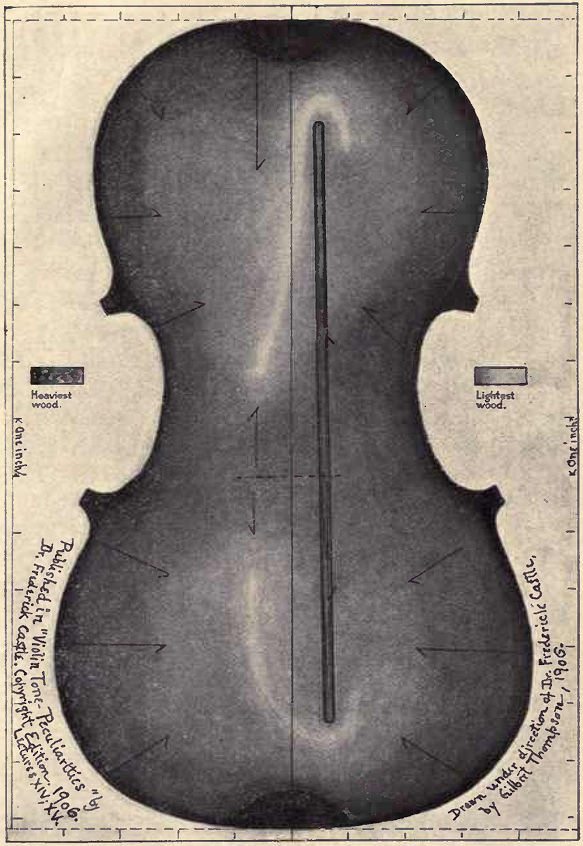
\includegraphics[width=1\textwidth]{./img/grafico.png} % Reemplaza "grafico.jpg" con el nombre del archivo de la imagen
\end{center}

\chapter*{Contenido}

\begin{itemize}
    \item \textbf{GRÁFICO} ... 6
    \item \textbf{ÍNDICE} ... 8
    \item \textbf{INTRODUCCIÓN} ... 12
    \item \textbf{CONFERENCIA I—Carácter del Tono del Violín} ... 17
    \item \textbf{CONFERENCIA II—Accidente Nº 1} ... 26
    \item \textbf{CONFERENCIA III—El Constructor de Violines Fraudulento} ... 42
    \item \textbf{CONFERENCIA IV—Madera de la Tabla Armónica del Violín} ... 57
    \item \textbf{CONFERENCIA V—Desintegración de las Superficies Interiores del Violín} ... 78
    \item \textbf{CONFERENCIA VI—Mi Violín Desgastado, o Fenómeno del Barniz Nº 1} ... 92
    \item \textbf{CONFERENCIA VII—Fenómeno del Barniz Nº 2} ... 113
    \item \textbf{CONFERENCIA VIII—Uniformidad de los Valores del Violín} ... 130
    \item \textbf{CONFERENCIA IX—Modificadores del Tono del Violín} ... 150
    \item \textbf{CONFERENCIA X—Modificadores del Tono del Violín, continuación} ... 160
    \item \textbf{CONFERENCIA XI—Modificadores del Tono del Violín, continuación} ... 171
    \item \textbf{CONFERENCIA XII—Modificadores del Tono del Violín, continuación} ... 180
    \item \textbf{CONFERENCIA XIII—Modificadores del Tono del Violín, continuación} ... 190
    \item \textbf{CONFERENCIA XIV—Uniformidad Máxima del Poder Tonal del Violín} ... 205
    \item \textbf{CONFERENCIA XV—Uniformidad Máxima del Poder Tonal del Violín, conclusión} ... 222
    \item \textbf{CONFERENCIA XVI—Poder Tonal Máximo del Violín} ... 235
    \item \textbf{CONFERENCIA XVII—Filosofía Relacionada con las Condiciones de las Superficies Interiores del Violín} ... 256
    \item \textbf{CONFERENCIA XVIII—Nuestro Pasar} ... 274
    \item \textbf{APÉNDICE} ... 289
\end{itemize}

\chapter*{Índice}

\begin{itemize}
    \item \textbf{ACCIDENTE Nº 1} ... 26
    \item \textbf{SONIDO AUDIBLE} limitado a doce pulgadas de la tabla armónica del violín, 53
    \item \textbf{ÁNGULOS} incidencia y reflexión, 304
    \item \textbf{LIBROS} evidencia poco confiable en, 35
    \item \textbf{MEJOR VIOLÍN SOLISTA} no el mejor violín de orquesta, 37
    \item \textbf{PLACA POSTERIOR} funciones de, 47; como un agente productor de tono, 107
    \item \textbf{CUIDADO DEL BARNIZ} ejemplo, 93
    \item \textbf{BARNIZ DE CREMONA} 125
    \item \textbf{EFECTO TONAL COMBINADO} media docena de violines de tono uniforme, 136; condiciones de la prueba, 136
    \item \textbf{TONO FRÍO} 296
    \item \textbf{SOBRETONOS DISONANTES} causa de, 30; 295
    \item \textbf{FRAUDE} 43
    \item \textbf{PROPÓSITO GENERAL} Violín, 38
    \item \textbf{GOMAS} duras, inelásticas, efecto de, 93
    \item \textbf{EL GUSHER} 285
    \item \textbf{ARMÓNICOS} valor de, 96
    \item \textbf{SOBRETONOS ARMÓNICOS} 294
    \item \textbf{INTRODUCCIÓN XII} método de llegar a conclusiones, xiv, ocho proposiciones, xv
    \item \textbf{INSENSATEZ} continuar la demanda de que solo aparezcan solistas con un Stradivarius o un Guarnerius, 39
    \item \textbf{INVITACIÓN} a mi violín de pastor, 101
    \item \textbf{LONGEVIDAD} del violín, 98; ejemplo, 98
    \item \textbf{PÉRDIDA DE PODER TONAL} causas de, 299
    \item \textbf{CONDICIONES METEOROLÓGICAS} 23
    \item \textbf{SONIDO MUSICAL} ley explícita, 30; afectando la distancia recorrida por el tono del violín, 280
    \item \textbf{UNIFORMIDAD MÁXIMA} del poder tonal del violín, 205; tonos fundamentales, 208; razones que conducen a un nuevo método para la graduación de la tabla armónica, 214; demostración de áreas de la tabla armónica que aumentan el tono de cada cuerda, 216; proporción para las longitudes de actividad de las fibras debajo de cada cuerda, 218; afinación de concierto hace 200 años, 223; demostración de que los errores en la graduación de la tabla armónica causan poder tonal desigual, 225
    \item \textbf{PODER TONAL MÁXIMO} 235; "gran" tono, 236; el tono del violín separado por dos factores irreconciliables, 237; esteticismo del violín llevado al extremo, 238; lista de factores que producen el poder tonal máximo del violín; apariencias físicas de la madera de la tabla armónica que produce un poder tonal máximo combinado con tono "rico", 246; vibración normal y transversal en la tabla armónica, 249; tono amaderado, 255; dispersión de la fuerza, la pelota rebotando, 271
    \item \textbf{RUIDO} definición de, 25
    \item \textbf{NODOS} 294
    \item \textbf{OH, TÚ POSTE} 276
    \item \textbf{TONO} Sonido musical, 30
    \item \textbf{INTÉRPRETES} Opiniones variadas de, 36
    \item \textbf{FILOSOFÍA} Involucrada en las condiciones de las superficies interiores del violín, 256; lista de principios que modifican el tono del violín, 259; número de cualidades tonales absolutamente al alcance del constructor de violines, 261; intensidad del tono del violín producto de cuatro factores, 262; propiedades del aire que afectan la intensidad del tono del violín, 264
    \item \textbf{PENETRACIÓN} del aceite, 274
    \item \textbf{PASAR} 276
    \item \textbf{POSTE} problema del, 301
    \item \textbf{TONO RICO} causas de, 96; descripción de la madera rica en tono, 97; ilustración, 296
    \item \textbf{CIENCIA} nunca hizo un violín, 32
    \item \textbf{DECLARACIONES CIENTÍFICAS} recibidas con precaución, 32
    \item \textbf{MADERA DE LA TABLA ARMÓNICA} 57; contribución de la ciencia, 58; valor en escrutinio de la madera usada, 61; violines desiguales, encogimiento, ejemplo, 62; ejemplo, 63; fallas del pino, 66; pino de Michigan, 67; cedro blanco, 69; cambios de color en el pino, 70, acción independiente de fibras contiguas, 71; patético, 78; preservando superficies interiores, 79; ejemplo de desintegración de superficies interiores, 83
    \item \textbf{ACCIÓN SIMPÁTICA} 108; ley de, 109
    \item \textbf{VIOLÍN ANTIGUO Y DULCE} 91
    \item \textbf{EL REY} 20
    \item \textbf{DOS ERRORES} 22
    \item \textbf{PRUEBA DE DISTANCIA DE TONO} al aire libre, 23; el oído escuchando en la mejor posición, 24
    \item \textbf{PROMOTORES DEL COMERCIO} industria de, 39
    \item \textbf{EL HOMBRE DE DOS DÓLARES} 41
    \item \textbf{TÚ, OH VIOLÍN} 45
    \item \textbf{ALTURA DEL TONO} 45; ocho reglas de aplicación, 48; regla 2, 48; regla 3, 49; regla 4, 49; regla 5, 50; regla 6, 50; regla 7, 51; regla 8, 51
    \item \textbf{MODIFICADORES DEL TONO} lista, 141; barniz, 142; doblado de la tabla armónica, 143; doblado de la parte posterior, 144; espesor de la tabla armónica, 144; arqueado, 147; arqueado alto, ejemplo, 148; leyes que gobiernan las líneas de viaje de las ondas sonoras, 151; problema no resuelto en el arqueado, 152; la barra, 152; lobo causado por mala posición de la barra, 153; lobo causado por la graduación, 154; posición de la barra disminuyendo el poder de la cuerda D, 158; el poste, 160; el puente, 164; el diapasón, 165; las cuerdas, 181; bloque de refuerzo, 175; el violín tembloroso, 181; superficies interiores, 185; las salidas, 187; profundidad de las costillas, 199; la sordina, 302; crines del arco, 202
    \item \textbf{UNIFORMIDAD} de los valores tonales del violín, 131
    \item \textbf{VEREDICTO} Etiqueta, Barniz y Precio vs Tono Dulce, 305
    \item \textbf{CARACTERÍSTICAS DEL TONO DEL VIOLÍN} lugar de utilidad, 19
    \item \textbf{TRABAJOS DE CHAPADO} 53
    \item \textbf{FENÓMENO DEL BARNIZ Nº 1} 104
    \item \textbf{FENÓMENO DEL BARNIZ Nº 2} 113
    \item \textbf{VIBRACIÓN} normal y transversal, 291; velocidad comparada, 299
    \item \textbf{SEGMENTOS VENTRALES} 295
    \item \textbf{LOBO} causado por la barra, ejemplo, 153; causado por la graduación de la tabla armónica, ejemplo, 154
\end{itemize}

\chapter*{Fe de Erratas}

\begin{itemize}
    \item Página 19, línea 8, en lugar de "tenora," lea tenoro.
    \item Página 44, línea 2 verso, en lugar de "Music," lea Music's.
    \item Página 48, línea 12, en lugar de "give," lea gives.
    \item Página 57, línea 24, en lugar de "govern's," lea governs.
    \item Página 96, línea 14, en lugar de "a basso," lea a bassa.
    \item Página 173, línea 1, en lugar de "diminish," lea increase.
    \item Página 216, línea 20, en lugar de "purfing," lea purfling.
    \item Página 217, líneas 1, 13, en lugar de "purfing," lea purfling.
    \item Página 297, línea 3, en lugar de "MOVEMENT," lea MOVEMENTS.
\end{itemize}

\chapter*{Introducción}

Estas conferencias, dirigidas a una audiencia imaginaria de estudiantes de violín, fueron originalmente escritas y parcialmente publicadas en el Western Musician, Dixon, Illinois, para el entretenimiento de los numerosos lectores de esta revista musical. Dos de las conferencias ahora aparecen impresas por primera vez. Como se empleó un estilo familiar, se evitaron términos técnicos abstractos en la medida de lo posible sin interferir con la claridad y precisión.

Los experimentos, resultados y conclusiones, tal como se registran aquí, no son fantasías de la imaginación, como podría inferirse al principio, sino que son conclusiones obtenidas a través de experimentos prácticos, y también por accidentes ocurridos en mi experiencia.

Así, cuando pacientes violines llegaron a mi hospital, me sentí feliz, y debido a mi entusiasta devoción a los problemas de diagnóstico tonal, trabajé sobre ellos, y sobre ellos, hasta declararlos curados o incurables. Algunos de esos pacientes violines eran, como algunos pacientes humanos, bendecidos con buenas constituciones inherentes desde el principio, y eran capaces de recibir valores tonales mejorados a partir del ajuste cuidadoso de los factores modificadores del tono, mientras que otros eran tan inherentemente malos desde el día en que fueron llamados "violín" (mal llamados), que solo heredaron un tono ruidoso; sin embargo, el tono ruidoso hizo "casos interesantes" de esta última clase debido a que ofrecían razones incontrovertibles para el tono inferior, razones que demostraban concluyentemente la verdad en la afirmación "sin material superior, sin violín superior."

Durante mi periodo de trabajo activo, siempre tuve en mente las siguientes preguntas:
\begin{itemize}
    \item "¿Cómo opera el violín para producir sonido musical?"
    \item "¿Qué agentes, conectados con el violín, operan para modificar el tono?"
    \item "¿Cuáles son las causas del tono inferior en un violín?"
    \item "¿Cuáles son las causas del tono superior en un violín?"
\end{itemize}

Algunas de estas preguntas las he resuelto a mi satisfacción, pero no pretendo que tales soluciones sean aceptables para otros estudiantes de fenómenos tonales del violín; ni pretendo que todos esos problemas de tono hayan recibido solución. Algunas de mis conclusiones están en desacuerdo con las conclusiones de investigadores científicos notables, pero no reclamo infalibilidad para mis propias conclusiones. Errar es humano. Seguir el error también es humano. Así, seguí una conclusión científica sobre la producción y modificación del tono del violín que requirió experiencias de veinticinco años para disipar la ilusión. Sobre esta base, se advierte al estudiante de violín sobre el peligro de seguir teorías abstractas bajo el disfraz de la ciencia.

Creo que las teorías, incluso cuando se basan en demostraciones prácticas repetidas en varios violines, deben presentarse solo como conclusiones de un individuo que intenta resolver un problema en el que la acción caprichosa de la madera ha sido, es y siempre puede seguir siendo una cantidad desconocida; y presento la idea de que tal cantidad desconocida es la razón por la cual la ciencia fracasa al intentar construir un violín por encargo.

Los siguientes problemas permanecen sin elucidación:
\begin{itemize}
    \item "Acción caprichosa inherente de la madera."
    \item "Diferentes grados de concentración de ondas sonoras en las salidas según diferentes grados de arqueado de las placas."
    \item "El fenómeno de elevar la altura tonal al agrandar el área de las salidas."
\end{itemize}

Se presenta la opinión de que las soluciones para los dos primeros problemas pondrán la calidad tonal del violín bajo el control de la voluntad. No obstante, a pesar de las dudas de resolver los problemas involucrados en la acción caprichosa de la madera, el valor de tal solución sigue siendo un incentivo poderoso para continuar el esfuerzo. El deseo de violines que posean un tono "rico" combinado con una marcada intensidad de tono es un estímulo que supera el estímulo del oro fino; y quien descubra un método para producir tales violines a voluntad se convertirá en un rey en su propio derecho.

Mi método para llegar a conclusiones sobre la potencia de cada modificador del tono del violín es investigar las causas del tono ruidoso, tono dulce, tono poderoso, tono hueco, tono fino, tono "todo por dentro", tono "todo por fuera", volumen de tono, intensidad del tono, altura tonal, tonos dobles no musicales, tonos abiertos poderosos con tonos altísimos débiles, tonos resultantes o armónicos a bassa, sobretonos consonantes, sobretonos disonantes, el "tono rico", el "tono frío", tono simpático, uniformidad del poder tonal, y carácter tonal basado en el carácter tonal de la voz humana.

En este trabajo, las conclusiones aquí presentadas siguen experimentos realizados tanto en violines antiguos como nuevos, y el número de tales violines asciende a cientos. A partir de las deducciones así obtenidas, mi deseo es dar prominencia a las siguientes proposiciones:
\begin{itemize}
 \item Las peculiaridades tonales que existen en un violín dado pueden no existir en ningún otro violín.
 \item Escribir sobre peculiaridades tonales que existen en un violín dado como necesidades infalibles para todos los violines es engañoso.
 \item Encontrar dos violines que posean valores tonales precisamente similares es igualmente difícil que encontrar dos voces que posean valores tonales precisamente similares.
 \item Ningún fabricante de violines, sea quien sea, ha sido capaz de otorgar un valor tonal destacado a cada violín.
 \item Que el pastor de ovejas de la montaña puede producir un violín con valores tonales iguales a los mejores.
 \item Que el mecánico hábil, guiado por un instinto musical infalible, produce un número vastamente mayor de violines superiores que el mecánico sin tal instinto.
 \item Que todos los fabricantes de violines pueden experimentar derrotas ocasionales.
 \item Que, salvo accidente, el violín superior es producto de una habilidad mecánica superior combinada con un sentido musical superior, todo dirigido sobre material superior.
\end{itemize}
No parece haber otro método que ofrezca un valor igual a las conclusiones que el método aquí presentado para determinar la potencia y operación de cada factor que interviene en la producción y modificación del tono del violín.

A la evaluación de tales factores he dedicado una vida; no en teorías abstractas, sino sentado en el banco mientras repetía demostración tras demostración, año tras año, década tras década, desde la juventud hasta la vejez, decidido a aislar, evaluar y conocer la operación de todos y cada uno de los factores subyacentes en los fenómenos tonales del violín, o morir en el intento. A los sesenta y tres años, la muerte estuvo cerca, y tres años después siguió cerca, dejando solo mi brazo derecho suficientemente útil para guiar la pluma. Ahora es seguro que no alcanzaré la meta de mi ambición.

Bajo tales dificultades, escribir es laborioso; además, el material aquí presentado se compone completamente de memoria, no se tomaron notas con vistas a la publicación. En el momento presente, la conservación necesaria de fuerzas me limita a un período diario limitado de trabajo; por lo tanto, abandono la reescritura planeada de la publicación preliminar, de la cual se hicieron las correcciones necesarias, y de la cual se omiten algunos párrafos, y a la cual se agregan las conferencias xvi y xvii. Esta publicación se presenta como mi legado tanto para el estudiante de violín como para el fabricante de violines estadounidense. Que el siguiente registro se reduzca a la escritura y se publique es algo debido enteramente al estímulo ofrecido por un fabricante de violines moderno; por lo tanto, cualquier entretenimiento o cualquier otro valor que se pueda encontrar en estas páginas es algo no atribuible únicamente al coraje de, FREDERICK CASTLE. Lowell, Indiana, 20 de marzo de 1906.

\chapter*{Conferencia I}
SEÑORES ESTUDIANTES DEL VIOLÍN, en esta, nuestra primera sesión, aprovecho la oportunidad para ofrecerles mis felicitaciones por los siguientes hechos interesantes. Primero: se han descubierto las causas del tono ruidoso en los violines. Segundo: se ha perfeccionado una forma exitosa de preservar las superficies interiores del violín de la desintegración por el calor y la humedad. Tercero: las áreas de la tabla armónica del violín, responsables de la producción y aumento del tono, han sido localizadas y definidas. Cuarto: se ha demostrado un método de graduación de la tabla armónica que asegura la máxima uniformidad en el poder tonal. Quinto: los principios que rigen la intensidad del tono del violín han salido a la luz. Sexto: los principios que gobiernan el poder del tono del violín se han expresado en palabras. Séptimo: se ha descrito la calidad de la madera de la tabla armónica que permite obtener un "tono rico" en el violín. Octavo: se ha registrado el poder del accidente para disipar la oscuridad y la ilusión. Noveno: algunas conclusiones científicas sobre "cómo opera el violín para producir sonido musical" han sido sacudidas. Décimo: se ha demostrado la falacia en la afirmación de que "los mejores Cremonas son vehículos necesarios para la interpretación de las partituras de Haydn, Mozart y Beethoven". Undécimo: se ha intentado corregir los agravios impuestos al fabricante de violines moderno por el "promotor del comercio de violines antiguos".

Durante nuestro curso de estudio, se les presentarán algunas ideas sobre el tono del violín que hasta ahora no se han expresado. De hecho, les prometo que habrá muy poco contenido repetido en nuestro menú. Como no es mi intención privarlos del placer que ofrece la anticipación, solo se les darán pequeñas dosis a la vez. Este plan se adopta para evitar dañar su capacidad de digestión y para asegurar su asistencia regular.

El gusto por el tono varía—varía a través de cada grado de cultura musical. Un tono que agrada a una persona puede no agradar a otra. Ningún intérprete puede tocar al máximo en un instrumento cuyo tono le resulte desagradable. Afortunadamente, el violín ofrece una variedad de calidad tonal tan infinitamente grande que cada violinista en la Tierra puede poseer uno con una calidad tonal que se ajuste a su gusto.

Uno podría pensar que es posible fabricar violines con un estándar único de calidad tonal, pero el hecho es que la peculiaridad inherente de la acción de la madera lo impide.

Existe algo que se aproxima a un estándar tonal invariable para toda la gama de instrumentos de viento e instrumentos de percusión.

Pero la calidad tonal invariable se detiene abruptamente ante la presencia de la familia del violín. Podemos imaginar la inmensa sorpresa de alguien que nunca ha escuchado otros instrumentos que no sean de viento al ser introducido a esta familia de violines. A medida que toma violín tras violín, viola tras viola, violonchelo tras violonchelo, no encuentra dos que posean un carácter tonal idéntico. Cada violín, cada viola, cada violonchelo tiene una calidad tonal peculiar a sí mismo. Estas peculiaridades son tan marcadas que pronto se vuelve capaz de nombrar cada violín con cuyos tonos está familiarizado, aunque esté con los ojos vendados o en una habitación distante, nombrándolos con la misma certeza con la que puede identificar diferentes cantantes con cuyos tonos está familiarizado.

Se vuelve curioso por conocer la razón o las razones de la infinita peculiaridad tonal de ese maravilloso instrumento musical llamado "violín".

Por observación, descubre que las cuerdas G y D a veces poseen un carácter tonal grave; en otros momentos, estas cuerdas poseen un carácter barítono-tenor; en algunos casos, las cuerdas A y E poseen un carácter mezzo-soprano; en otros casos, las cuerdas A y E poseen únicamente un carácter soprano.

Debido a estas peculiaridades tonales, clasifica los violines en cuatro categorías, de la siguiente manera:

Basso-mezzo-soprano.
Basso-soprano.
Barítono-mezzo-soprano.
Barítono-soprano.
Por experimentación, descubre que estas cuatro clases de carácter tonal pueden ser dadas a los violines a voluntad, y que dependen de diversos grados de espesor de la tabla armónica, junto con modificadores del tono como el tamaño y la posición de las salidas, la capacidad de aire del violín, etc.

Por observación, encuentra un campo de utilidad peculiar en dos de estas clases. Así: El violín con carácter tonal basso-mezzo-soprano es el instrumento solista más agradable, mientras que el violín con carácter barítono-soprano es decididamente más efectivo para su uso en la orquesta; este último hecho se debe a la alta altura tonal, lo que permite que sus ondas tonales se sitúen sobre las ondas de las demás partes armónicas.

Sorprendentes como son estas peculiaridades, aún encuentra otro hecho en el tono del violín aún más sorprendente; es decir, algunos violines poseen una calidad tonal humana en un grado muy superior a todos los demás dispositivos musicales. Así, se le abre un nuevo mundo de expresión.

Aquí tenemos un dispositivo musical capaz de "hablar"; capaz de participar en un diálogo al estilo del "Arkansas Traveler", un instrumento capaz de detener el canto de las aves silvestres, haciendo que, con el cuello extendido y los ojos iluminados por la maravilla, busquen a ese otro extraño "cantante" que emite esos trinos encantadores; un instrumento capaz de estallar en risas alegres al estilo de la partitura de risas en el "Carnaval" de Paganini; un instrumento capaz de pronunciar oraciones devotas en la "Canción sin Palabras" de Mozart; un instrumento que llena el aire con esos tonos que hacen olvidar los problemas en el "Sueño" de Schumann; que despierta la ternura humana con los tonos simpáticos de "Sweet Home"; que hace llorar a los ojos humanos con esos incomparables, conmovedores y desesperados tonos de despedida, como la valiente, amorosa e inquebrantable Norma, condenada a muerte en la hoguera por su severo padre druida, cantando en el "Duetto e Scena Ultima" mientras asciende a esa pira funeraria ardiente—¡Dios mío! ¡Qué lágrimas cegadoras! ¡Qué agonía!

En todo el amplio mundo, no hay ningún instrumento musical que se acerque al violín. Nuestro investigador del violín se ha convertido ahora en un devoto del violín. Los tonos encantadores de este prodigio afinado a la humanidad lo obligan a inclinarse y adorarlo como "El Rey".

¡Tú, oh violín!
¡Tú, que sonríes tanto al mendigo como al rey!
Tú, cosa que ríes, lloras, rezas, cantas!
¡Tú, cosa de belleza!
¡Tú, alegría eterna!
Ni reyes, ni reinas, ni potentados
Reinan con tu absolutismo.
¡Tú, oh violín!

¿Condenas a este hombre por tal adoración idólatra?

He dedicado más de cincuenta años a la búsqueda de las causas de las peculiaridades tonales del violín; encontrando algunas de ellas, o eso creo. No reclamo un conocimiento superior de la física, ni una penetración superior. Solo reclamo mérito por mi tenacidad.

El fisionomista podría decir de mí: "tienes una mandíbula cuadrada". El frenólogo podría decir: "tienes un desarrollo notable en la región de no-dejar-ir". Ambos podrían concluir diciendo: "no tienes nada más digno de mención". Solo la tenacidad puede mantener a un hombre trabajando durante cincuenta años en un solo problema.

Trabajé cuarenta años intentando que todos los violines tuvieran un tono dulce; en otras palabras, intentando encontrar la causa del "ruido" en el tono del violín. Había llegado a la conclusión de que el tono dulce en el violín es un accidente, cuando ocurrió un verdadero accidente que reveló la causa del ruido en menos de diez minutos.

¿Ironía?
Mucha.
Confieso que una solución por accidente es mejor que ninguna solución. Cuando un hombre, incluso con la ayuda de un accidente, vive para demostrar un principio beneficioso para la humanidad, puede partir sabiendo que el mundo es mejor por su existencia.

¿No es un hecho que cuando un hombre puede elevar a la humanidad por encima del ruido desgarrador, desolador y suicida del violín, tiene suficiente base para cualquier reclamo razonable en la Tierra o en el cielo?

Que lo atestigüen millones de personas con "nervios".
¡Basta!

Algunos violines tienen un tono dulce; otros no.
La verdad es que pocos violines son realmente dulces; muchos no lo son.
Para el oído atento, la dulzura es el principal elemento de valor en el tono del violín. Curiosamente, hay algunos violinistas que no le dan valor a la dulzura del tono, diciendo: "me encargaré de la dulzura si logro obtener poder tonal".

Nunca ha habido un error mayor.
Los mejores violinistas, desde Ole Bull hasta el Sr. "Sierra-tu-cabeza", no podían, ni podrán jamás, ocultar el tono "ruidoso" de un violín. Admitiendo una diferencia a favor de la técnica hábil con el arco, aun así, por muy hábil que uno sea, el noventa por ciento del público dirá: "Ese sujeto no sabe tocar el violín".

Por tono dulce me refiero a un tono no acompañado de ondas sonoras afinadas en claves inarmónicas.

Además, es un error suponer que el "tono ruidoso" viaja la misma distancia que el tono dulce. En este punto, la siguiente prueba de alcance ofrece al devoto del tono fuerte una buena oportunidad de desilusión, y también de desprenderse de su riqueza. Es una prueba que he realizado repetidamente, con resultados invariantes.

Como bien saben, un violín de tono fuerte y ruidoso, tocado en una habitación pequeña y desnuda, hace que uno anhele la tranquilidad de un bosque sombreado. De una serie de violines probados en una habitación pequeña, seleccionen el más ruidoso y el más dulce, y llévenlos a un campo abierto, nivelado, que ofrezca al menos 1400 pies lineales de distancia sin obstrucciones. Seleccionen un día sin viento; un día despejado es el mejor, porque cualquier cosa que se acerque a una nube nimbos ayuda mucho en la propagación del sonido. Elijan una hora entre las 10 a. m. y las 4 p. m., ya que en esas horas del día el sonido se propaga con mayor dificultad. Para que el registro tenga valor, lleven un termómetro, un barómetro y un higrómetro, y registren las lecturas de estos instrumentos en el momento de la prueba. Así, el poder de alcance de un violín probado de esta manera puede garantizarse para repetir su rendimiento en cualquier momento bajo condiciones meteorológicas similares. Como saben, las condiciones meteorológicas modifican en gran medida las distancias a las que viaja el sonido. En nuestros meses de verano, estas condiciones a menudo hacen que el tono del violín sea decepcionante. Por lo tanto, cualquier violín puede ser objeto de una crítica tonal injusta.

Al realizar esta prueba de distancia tonal, al menos dos personas deben asistir.
Una tocará una melodía en la cuerda G; la otra se retirará a través del campo hasta una distancia en la que la melodía se distinga débilmente. Esta distancia, medida, se acreditará a esa cuerda. Así se registrará cada cuerda de cada violín.

Esta prueba establece:
\begin{itemize}
 \item Uniformidad del poder tonal.
 \item Intensidad del tono. (Poder de alcance).
 \item Pureza del tono. (Dulzura del tono).
\end{itemize}

En mi experiencia, el tono más dulce viaja invariablemente una mayor distancia. He conocido a violines de tono más dulce que han ganado por 250 pies. En uniformidad del tono, probé un violín antiguo reputado cuyo registro de distancia varía de 1000 pies para la cuerda G a 1480 pies para la cuerda E. Solo he probado dos violines de esta manera, obteniendo un registro de distancia igual para cada cuerda.

Les aseguro que esta prueba de distancia del tono puede causar una profunda sorpresa a los participantes. Yo mismo, después de una larga experiencia, no me atrevo a arriesgarme con el resultado. Esta prueba proporciona una prueba amplia de que el oído atento está en la mejor posición para juzgar el tono.

En este punto presento el "ruido". 
Es algo familiar, verdaderamente. 
Es algo que no debería encontrarse en el violín. 
No siempre en los libros de texto encontramos una definición de "ruido". 
El ruido parece ser un tema doloroso. La proximidad acentúa su dolor.

La existencia del "ruido" es como la densidad de población. Al ruido se le puede achacar la existencia de "nervios". Este hecho puede ser probado al retroceder unos siglos, cuando había menos personas en la Tierra, menos cosas en movimiento y muchos menos violinistas, y allí no encontramos registro de "nervios". La ciencia nos haría creer que donde no hay oídos, no hay sonido, no hay "ruido".

¿Creen en esta historia? Si no desean expresar su incredulidad, al menos pueden llamarla una paradoja. ¡Pero pensar en un lugar donde no haya ruido! ¡Lugar bendito! ¡Debe ser un lugar donde los ángeles no temen pisar! Que no sea invadido por el violín "ruidoso", ya que el ruido más desconcertante, el ruido "le plus terrible", puede provenir del violín.

¿Qué es el ruido? Si no encuentran una definición que les convenga, lean lo siguiente: El ruido es una agregación de ondas sonoras afinadas en teclas inarmónicas.

La definición misma provoca escalofríos. Estoy orgulloso de ello; del escalofrío, me refiero. El escalofrío es prueba de que mi definición es correcta.

¿Cuál es la causa del "ruido" en el tono del violín? Esta pregunta está llena de un interés absorbente para todo el mundo del violín. El accidente que proporciona una solución a esta importante pregunta es tan provocadoramente accidental que me roba todo honor por la solución.

He trabajado toda una vida en esta solución; he leído libros, y libros; he comprado algunos libros por mí mismo; he tomado prestados más. He aprendido allí algunos hechos que requirieron veinte y cinco años para desaprender; había renunciado a la posibilidad de una solución, creyendo que la dulzura del tono del violín era un accidente, cuando ocurrió el siguiente accidente, así:

\chapter *{Conferencia II}
\section*{Caballeros:}

Estaba trabajando en un violín usado, un violín con fallos de tono "ruidoso", un violín perteneciente a un intérprete "profesional". La re-graduación estaba completada, una nueva barra ajustada, el trabajo de acabado en las superficies interiores finalizado y todo listo para ensamblar cuando el propietario envió una solicitud de "apresúrate". Apresurarse significaba trabajar de noche, y para complacer a mi amigo, decidí realizar el trabajo de ensamblaje esa misma noche.

Por lo tanto, regresé a mi taller, encendí una lámpara de 20 vatios colocada frente a un reflector y me senté justo delante de la lámpara. Alcanzando con mi mano derecha, tomé la tabla armónica terminada. Al colocarla entre mi vista y la lámpara, noté algunas manchas oscuras en la superficie interior. Pensando que de alguna manera había ensuciado la superficie, dejé la tabla armónica, con la intención de eliminar esas manchas con un paño. Pero, cuando la tabla armónica quedó sobre el banco, no se veían manchas; habían desaparecido. La superficie interior estaba clara y brillante. Pero, ciertamente había visto manchas oscuras. Nuevamente sostengo la tabla armónica hacia la lámpara. Ahí están, claramente visibles; varias de ellas; algunas grandes, otras pequeñas. Deben ser causadas por manchas en la superficie barnizada. Examino críticamente el barniz. No aparecen manchas en la superficie barnizada. Posiblemente estas manchas podrían deberse a opacidades en la madera, pero no encuentro opacidades; la madera es clara y brillante. Nuevamente sostengo la tabla armónica hacia la lámpara. Una, dos, tres, seis áreas nubladas están allí, y ubicadas en la zona superior productora de tono de la tabla armónica.

Inmóvil, observo esas áreas nubladas, pensando, pensando profundamente en una explicación. Lentamente, la explicación vino, lentamente, por supuesto. No soy brillante; nunca me he presentado como un prodigio; soy lento, pero persistente, además soy fumador. Como saben, fumar es un requisito del filósofo. No podemos disociar la pipa del alemán, ni el mundo puede igualarlo en la resolución de problemas difíciles. Siguiendo el ejemplo del filósofo, encendí mi pipa. De inmediato, a través de nubes de humo, veo la causa de esas áreas nubladas. Así es como el "humo" ayuda a la filosofía.

El gran Hahnemann estableció el principio de que "lo similar cura lo similar"; o, como Hahnemann afirma en su elegante latín, \textit{“Similia similibus curantur”}. Yo creo en Hahnemann en lo que respecta al "humo"; sin embargo, ese gran pensador sí logró perforar la gruesa piel de los doctores "convencionales" con el hecho contundente de que nuestras dosis a menudo superan la generosidad. Y ahora yo, uno de los "convencionales", voy a demostrar que lo "infinitesimal" también puede causar "ruido" dentro del violín.

Creo en los accidentes. A su debido tiempo, les presentaré dos ocurrencias accidentales que apuntan directamente a la solución de problemas de tono en violines que hasta ahora se habían considerado insolubles. Por lo tanto, cuando me encuentro con preguntas imposibles de resolver, rezo por un accidente.

Si no hubiera sido por llevar accidentalmente esta tabla armónica con su superficie convexa hacia la lámpara, todavía podría estar buscando la causa del "ruido" en el tono del violín; es más, podría nunca haber encontrado la causa. En la siguiente narración, podrán ver claramente la evidencia innegable proporcionada por el accidente, porque, a la luz de las teorías del sonido musical, esta evidencia se presenta de manera clara y precisa.

Para que mi proceso de razonamiento quede claro, recordaré algunos hechos familiares de la filosofía natural: Así, los rayos de luz, al caer sobre la superficie convexa de un cuerpo cóncavo-convexo (como la tabla armónica del violín), después de atravesar dicho cuerpo se desvían de una línea recta en el momento de salir de la superficie cóncava, y de allí viajan en líneas convergentes hacia un foco; por lo tanto, los objetos sobre la superficie cóncava se magnifican; pero, al invertir la dirección de viaje, los rayos de luz que salen de la superficie convexa se dispersan; de ahí que los objetos sobre la superficie convexa parecen reducirse en tamaño. Por lo tanto, si hubiera llevado esta tabla armónica con su superficie convexa hacia la lámpara, no habría visto esas áreas nubladas. [El barniz transparente sobre la superficie convexa de esta tabla armónica facilita en gran medida la transmisión de los rayos de luz; y, al aplicar esta prueba para la graduación perfecta—trabajo sobre la madera de la tabla armónica "en blanco"—es necesario primero cubrir la superficie convexa con algún medio transparente, como aceite o barniz transparente, o mejor, una mezcla de estas dos sustancias disponibles.]

Al realizar el trabajo de graduación sobre esta tabla armónica, supuse que estaba haciendo un trabajo fino; utilizando los calibradores de manera cuidadosa; sin embargo, no había logrado un trabajo perfecto, como ahora se demostrará. Si esta tabla armónica hubiera sido ensamblada sin descubrir esas áreas nubladas, el tono habría estado mezclado con ondas sonoras afinadas en notas disonantes o "ruido". Como antes, sostengo la tabla armónica hacia la lámpara y, con un lápiz, circunscribo una de esas áreas y, en ella, con un raspador, elimino un poco de madera. Ahora, en esta área, la luz pasa más libremente. Continúo así con el raspador hasta que esta área circunscrita se vuelva igualmente luminosa que las áreas adyacentes.

\textit{"Doctor, ¿cuánta madera removió?"}

No puedo responder a esta pregunta con precisión, pero diría quizás la centésima parte de una pulgada en algunos lugares; en otras áreas de mayor opacidad, una cantidad mayor. Deben entender que la forma de graduación aplicada a esta tabla armónica es de 9/64 de pulgada en la posición del puente; de allí, en dirección ascendente o descendente, disminuye a 3/32 de pulgada en el borde, lo más cerca posible al trabajar. Por lo tanto, la precisión absoluta en la disminución de los espesores de la tabla armónica se vuelve un asunto difícil; de hecho, esta forma de graduación de la tabla armónica no es superada en dificultad por ninguna otra forma conocida. También deben entender que, donde el espesor es de 9/64, pasa poca o ninguna luz; también, que la mayor luminosidad, en esta placa, ocurre con un espesor de 3/32 de pulgada; y que, entre estos dos puntos, la luminosidad disminuye o aumenta con una regularidad exactamente proporcional a la disminución o aumento del espesor de la tabla armónica; por lo tanto, las irregularidades en el espesor producen áreas nubladas al interferir con el paso de los rayos de luz. Recuerdo las reglas que gobiernan la altura tonal. Me viene a la mente el hecho de que las irregularidades de una centésima de pulgada en una lengüeta de órgano, en un tubo de órgano o en un diapasón son inadmisibles. ¿Es también inadmisible tal irregularidad en la tabla armónica del violín? ¿He encontrado, finalmente, la causa del "ruido" en el tono del violín? Mis nervios están de punta. Cuarenta años he trabajado en violines usados tratando de encontrar una fórmula para erradicar el "ruido" de ellos; trabajando con la cantidad habitual de fracaso "ruidoso". Más rápido de lo que puedo contar, la inteligencia fue transmitida a mi sensorium de que esas ligeras irregularidades en el grosor de la tabla armónica podrían producir un tono chillón, penetrante, angustiante, de altura tonal inmensurablemente alta; un tono así para cada irregularidad en el área productora de tono de la tabla armónica del violín.

Han escuchado cómo los "prospectores" pueden "prospectar" durante toda una vida sin encontrar una "veta"; cómo, cuando encuentran una, inmediatamente celebran el evento volviéndose locos.

Caballeros: El tono de este violín no está acompañado por ondas sonoras afinadas en claves inarmónicas; y ahora conocen la causa del "ruido" en el tono del violín. En relación con la palabra "violín", la palabra "ruido" evoca vívidamente un sufrimiento incalculable; por lo tanto, no presionaré más este tema de lo necesario para la completa comprensión de esos sobretonos agudos, disonantes, que provienen de la tabla armónica imperfecta de un violín.

La ciencia afirma que el sonido musical se compone, en altura tonal, desde 27 hasta 4000 vibraciones por segundo; y, dado que el "ruido" del violín es exasperantemente agudo, se sigue que el "ruido" del violín posee una altura tonal que supera las 4000 vibraciones por segundo.

\end{document}
